% =============================================================================
% Chapter 11: Evaluation
% =============================================================================
\chapter{Evaluation}
\label{ch:evaluation}

\begin{objectives}
    \item Understand perplexity as an evaluation metric
    \item Compute perplexity on validation data
    \item Perform qualitative evaluation through generation
    \item Detect and prevent overfitting
\end{objectives}

% -----------------------------------------------------------------------------
\section{Perplexity}
% -----------------------------------------------------------------------------

\textbf{Perplexity} is the standard metric for language models.

\subsection{Definition}

Perplexity is the exponential of the average cross-entropy loss:

\begin{equation}
\text{PPL} = \exp\left(-\frac{1}{N}\sum_{i=1}^{N} \log p(x_i | x_{<i})\right) = \exp(\mathcal{L})
\end{equation}

\subsection{Interpretation}

Perplexity can be thought of as ``effective vocabulary size'':
\begin{itemize}
    \item PPL = 10 means the model is as uncertain as choosing from 10 equally likely tokens
    \item PPL = 100 means choosing from 100 equally likely tokens
    \item \textbf{Lower is better}
\end{itemize}

\subsection{Typical Values}

\begin{table}[H]
\centering
\begin{tabular}{ll}
\toprule
\textbf{Model/Dataset} & \textbf{Perplexity} \\
\midrule
Random (vocab=16K) & 16,384 \\
Untrained TryLM & $\sim$16,000 \\
Trained TryLM (TinyStories) & 20--40 \\
GPT-2 (WebText) & $\sim$20 \\
\bottomrule
\end{tabular}
\caption{Typical perplexity values}
\end{table}

% -----------------------------------------------------------------------------
\section{Computing Perplexity}
% -----------------------------------------------------------------------------

\begin{lstlisting}[style=python, caption={Perplexity computation from evaluate.py}]
@torch.no_grad()
def compute_perplexity(
    model: GPT,
    dataloader: DataLoader,
    device: str,
    max_batches: int | None = None,
) -> float:
    model.eval()
    total_loss = 0.0
    total_tokens = 0

    for i, batch in enumerate(dataloader):
        if max_batches and i >= max_batches:
            break

        batch = {k: v.to(device) for k, v in batch.items()}
        outputs = model(**batch)
        loss = outputs["loss"]

        # Count non-padding tokens
        mask = batch["labels"] != -100
        num_tokens = mask.sum().item()

        total_loss += loss.item() * num_tokens
        total_tokens += num_tokens

    avg_loss = total_loss / total_tokens
    perplexity = math.exp(avg_loss)

    return perplexity
\end{lstlisting}

\subsection{Using the CLI}

\begin{lstlisting}[style=shell]
uv run trylm eval --checkpoint checkpoints/best

# Output:
# Validation Perplexity: 28.45
\end{lstlisting}

% -----------------------------------------------------------------------------
\section{Qualitative Evaluation}
% -----------------------------------------------------------------------------

Numbers don't tell the whole story. Generate samples to assess quality.

\subsection{Sample Prompts}

\begin{lstlisting}[style=python]
prompts = [
    "Once upon a time",
    "The little girl",
    "One day, a boy named",
]

for prompt in prompts:
    output = generate(model, tokenizer, prompt, max_new_tokens=100)
    print(f"Prompt: {prompt}")
    print(f"Output: {output}\n")
\end{lstlisting}

\subsection{What to Look For}

\begin{itemize}
    \item \textbf{Grammar}: Are sentences well-formed?
    \item \textbf{Coherence}: Does the story make sense?
    \item \textbf{Creativity}: Is it interesting or just repetitive?
    \item \textbf{Completion}: Does it reach a natural ending?
\end{itemize}

% -----------------------------------------------------------------------------
\section{Train vs. Validation}
% -----------------------------------------------------------------------------

Compare perplexity on training and validation data:

\begin{itemize}
    \item \textbf{Similar}: Model generalizes well
    \item \textbf{Train << Val}: Overfitting (memorizing training data)
    \item \textbf{Both high}: Underfitting (model too small or undertrained)
\end{itemize}

\begin{figure}[H]
\centering
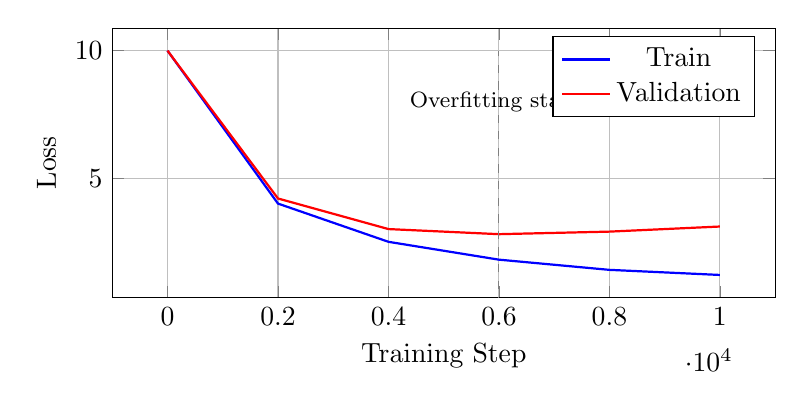
\begin{tikzpicture}
    \begin{axis}[
        width=10cm,
        height=5cm,
        xlabel={Training Step},
        ylabel={Loss},
        legend pos=north east,
        grid=major,
    ]
        \addplot[thick, blue] coordinates {
            (0, 10) (2000, 4) (4000, 2.5) (6000, 1.8) (8000, 1.4) (10000, 1.2)
        };
        \addlegendentry{Train}

        \addplot[thick, red] coordinates {
            (0, 10) (2000, 4.2) (4000, 3.0) (6000, 2.8) (8000, 2.9) (10000, 3.1)
        };
        \addlegendentry{Validation}

        \draw[dashed, gray] (axis cs:6000, 0) -- (axis cs:6000, 10);
        \node[font=\footnotesize] at (axis cs:6000, 8) {Overfitting starts};
    \end{axis}
\end{tikzpicture}
\caption{Detecting overfitting: validation loss increases while training loss decreases}
\label{fig:overfitting}
\end{figure}

% -----------------------------------------------------------------------------
\section{Summary}
% -----------------------------------------------------------------------------

\begin{summary}
    \item \textbf{Perplexity} = $\exp(\text{loss})$; lower is better
    \item Perplexity represents ``effective vocabulary size'' of uncertainty
    \item \textbf{Qualitative evaluation} through generation catches issues metrics miss
    \item Compare \textbf{train vs. validation} loss to detect overfitting
    \item Good TryLM performance: PPL 20--40 on TinyStories validation
\end{summary}
